\documentclass[fleqn,a4paper,11pt]{article}
\title{Pesten}
\author{Izaak van Dongen}

\usepackage{mysty}

\begin{document}
    \maketitle\thispagestyle{empty} % no page number under title
    \tableofcontents
    \lstlistoflistings

    \section{Introduction}

    Pesten is a classic Dutch card game, similar to Uno but played with playing
    cards. The name translates as something like `bothering'. The objective is
    to annoy your fellow players as much as possible. The suits function as
    colours, and various cards have special functions. There is also a fine
    tradition of introducing house rules.  People can feel very strongly about
    these, and we're still finding special cases that require and appeal to the
    van Dongen jury, so while this implementation aims to codify the van Dongen
    house rules, it makes no guarantee of absolute accuracy.

    It is played with one to two packs of cards, but this is entirely variable
    depending on how many players there are.

    \section{Rules}

    \subsection{Basic play}

    The basic functioning of the game is, as mentioned, very similar to Uno.
    There is a discard pile and a pickup pile. The top card of the discard pile
    determines the current player's allowable discards. A player is allowed to
    play any card of either the same suit or the same rank as the current card,
    or a joker, unless there is currently a special effect in play\ldots

    If a player is able to play, they must. However, if they can't, they pick
    up one card from the draw pile. If they are able to play this card, they
    may, and this card takes effect as normal.

    \subsection{Special cards}

    Some cards have effects, which generally apply to the next player. Due to
    this, sometimes players opposite each other form `teams' as they never
    obstruct each other. This mode of play also allows everyone to win more
    often. All effects are listed here:

    \begin{center}
    {
    \renewcommand{\arraystretch}{2.0}
    \begin{tabular}{lp{0.8\linewidth}} \toprule
    Card & Effect \\ \midrule
    Joker &
    This card has no suit so can be played on any card (unless this table
    specifies otherwise, see 2). The following player must take 5 cards, or
    play their own joker, which increases the count to 10 and moves to the next
    player. The player who ends up taking the cards may decide on the initial
    suit after the joker, but may not play. Play goes to the next player after
    the suit has been decided. \label{card:joker}
    \\ 2 &
    The following player must take 2 cards. If the following player has a 2,
    they may play it and then the total number of cards to be taken is 4, by
    the next player, and so on. A player may also `escalate' by playing a 3 of
    the same rank. This increases the payload by three. A following player must
    then play a 4 of the same rank or a 3, and so on. Any cards played in this
    mode are exempt from their normal special effects. A joker cannot be played
    while a 2-stack is in play. The player who ends up taking the cards may not
    play, and play goes to the next player from them.
    \\ 7 &
    A 7 allows the player to take another turn. Their next card must fit on
    the seven, or they will have to pick up a card.
    \\ 8 &
    An 8 skips the next player. This action cannot be stopped by any card,
    as the next player simply doesn't get a turn, so cannot do anything like
    play their own 8.
    \\ 10 &
    A 10 means the player before the current player now has their turn, but
    play goes on as normal.
    \\ Jack &
    A jack lets the player choose the suit to go on with. The next player must
    play a jack, or a card of the declared suit, or a joker.
    \\ King &
    Changes the direction of play. The next turn goes the player originally
    `before' the current player.
    \\ \bottomrule
    \end{tabular}
    }
    \end{center}

    Any unmentioned cards are not special.

    \subsection{Card sets} \label{rule:sets}

    A player may also play a `set' of cards. A set of cards is either three or
    more of the same rank, or three or more adjacent cards of the same suit in
    ascending or descending order. For example, one might play
    \(6\ \clubsuit, 6\ \diamondsuit, 6\ \spadesuit\), or
    \(6\ \clubsuit, 5\ \clubsuit, 4\ \clubsuit\). NB for the purpose of these
    sets, aces are considered to be both before 2 and after the King.

    A set must contain at least three cards following the pattern. However, the
    play of two cards is permitted if they form a set with the top card on the
    discard pile, eg you can play \(6\ \diamondsuit, 6\ \spadesuit\) if there is a
    \(6\ \clubsuit\) at the top of the discard pile.

    If there are special effect cards, only the top card has its effect. This
    means that it's a better idea to play
    \(9\ \clubsuit, 8\ \clubsuit, 7\ \clubsuit\)
    than the other way round, as this gives the player another turn.

    If a card set is played while a 2-stack is building, only the last card of
    the set contributes to the number to be picked up.

    \subsection{Last (card), but not least} \label{rule:lastcard}

    As soon as a player reaches their last card, they must tap the table twice
    and declare `last card' with appropriate volume and enthusiasm. If they
    don't, a two-card penalty is inflicted. If the player is playing a series
    of cards (using 7s, or sets) and they forget last card, they take back
    their last card and two penalty cards. They may not continue to play.

    \section{Class hierarchy}

    Here is my wonky UML:

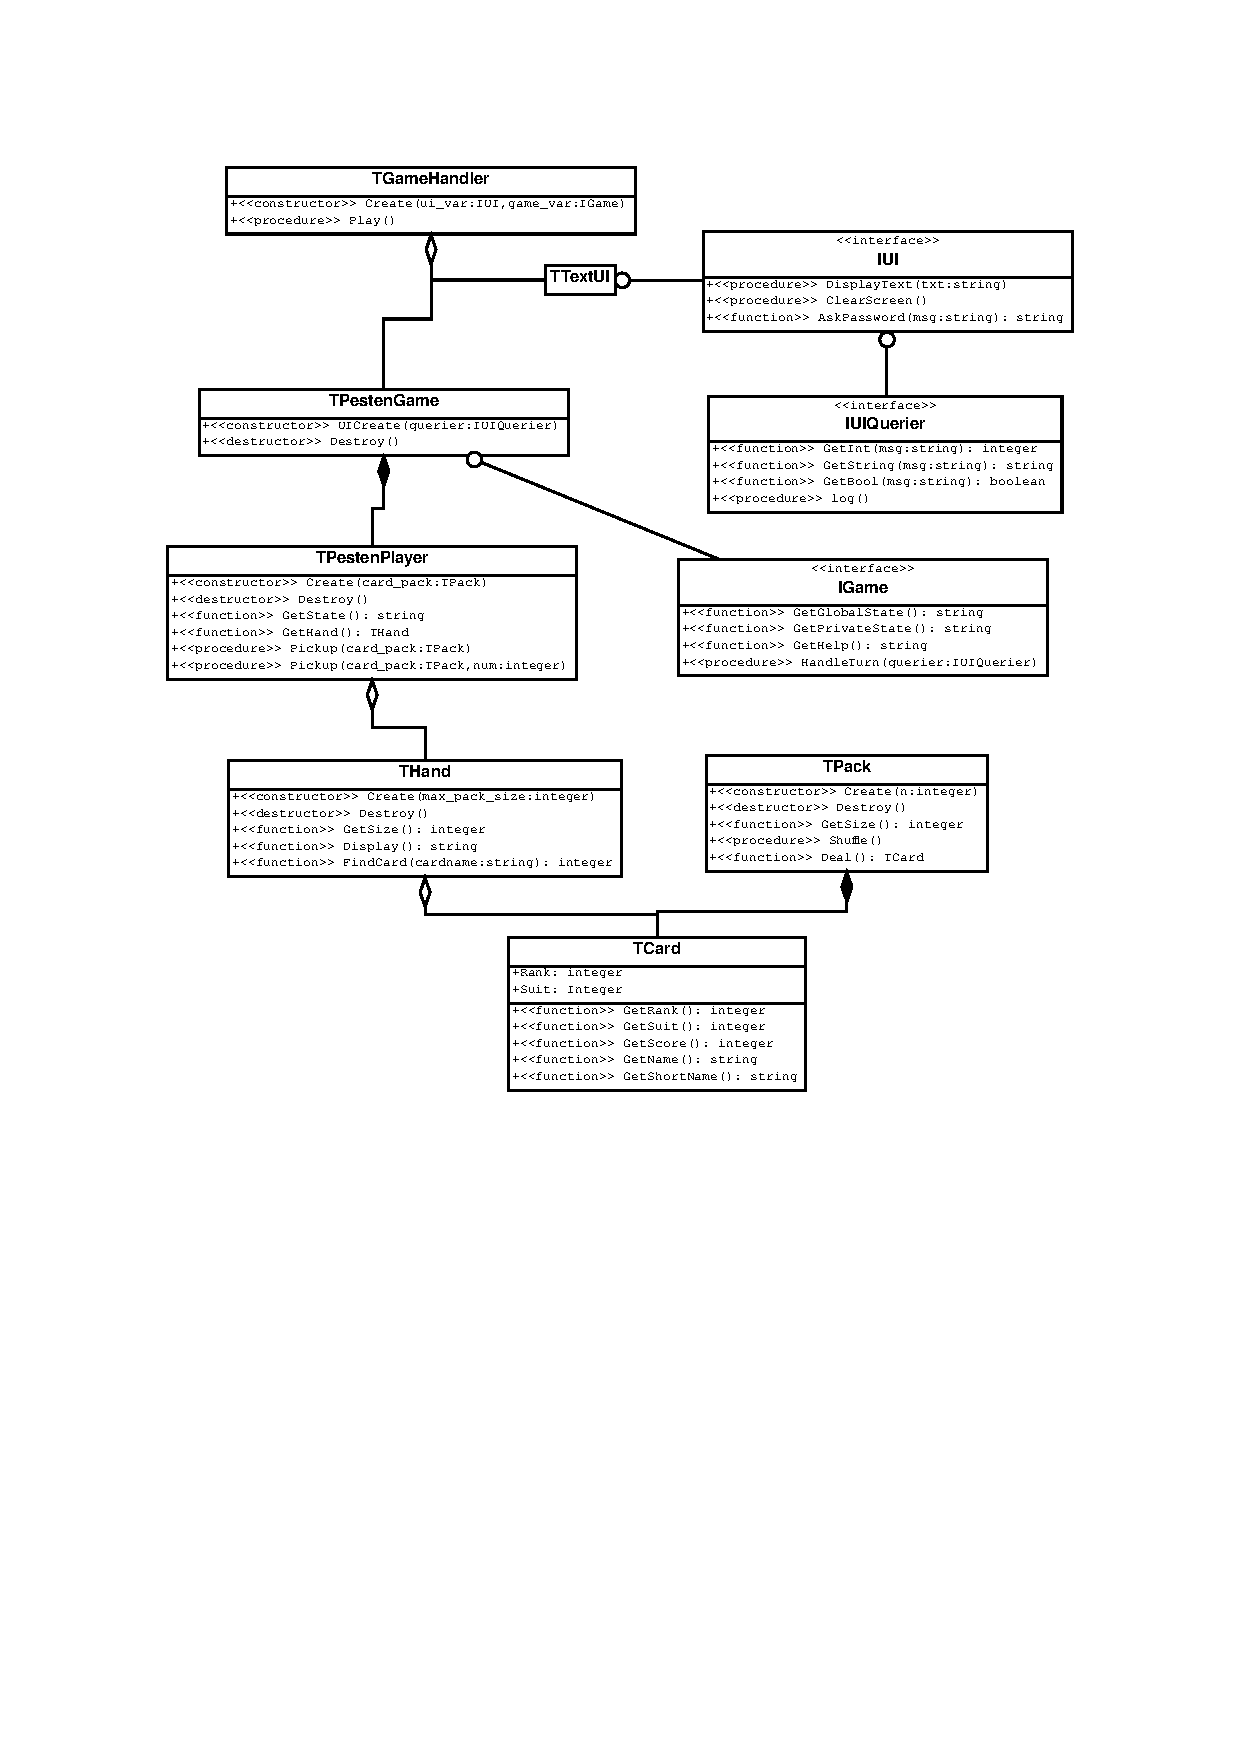
\includepdf[pages=-]{classes.pdf}

    \section{Implementation}

    All source code in Pascal and \LaTeX\ can be found at
    \url{https://github.com/goedel-gang/pesten}.

    This assignment's total source clocs
    \footnote{Count Lines of Code \url{https://github.com/AlDanial/cloc}.  This
    waffle was included for the pun and because I wanted to see if I could load
    the loc count into a \LaTeX\ engine at compile time. Turns out I can.}
    in at
    \input{|"cloc ../src | gawk --field-separator ' +' '/^SUM/{print $NF}'"}loc
    (this \TeX\ document is an extra
    \input{|"cloc . | gawk --field-separator ' +' '/^TeX/{print $NF}'"}loc).

\lstinputlisting[language=Pascal, caption=UCard.pas]
{../src/UCard.pas}
\lstinputlisting[language=Pascal, caption=UPack.pas]
{../src/UPack.pas}
\lstinputlisting[language=Pascal, caption=UHand.pas]
{../src/UHand.pas}
\lstinputlisting[language=Pascal, caption=UUIQuerier.pas]
{../src/UUIQuerier.pas}
\lstinputlisting[language=Pascal, caption=UGame.pas]
{../src/UGame.pas}
\lstinputlisting[language=Pascal, caption=UPlayer.pas]
{../src/UPlayer.pas}
\lstinputlisting[language=Pascal, caption=UUI.pas]
{../src/UUI.pas}
\lstinputlisting[language=Pascal, caption=UGameHandler.pas]
{../src/UGameHandler.pas}
\lstinputlisting[language=Pascal, caption=PPesten.pas]
{../src/PPesten.pas}

    \section{Usage}

\begin{lstlisting}[caption=Initialisation routine]
How many packs?
Enter integer > 2
Which player number deals?
Enter integer > 1
How many players?
Enter integer > 3
\end{lstlisting}

    After this point the program sends the terminal the escape code for screen
    clearance, so an empty screen appears:

\begin{lstlisting}[caption=User taking a turn]
This is pesten, see the pdf. Cards denoted as ([23456789TJQKA][SCHD]|take)
history:
Game start
Game start
Game start
Game start
Game start
Player 1 plays a Six of Hearts
Top of discard is Six of Hearts

Your hand is: Hand(6C, 3H, 2D, 9H, KD, TH, 7D)
What card would you like to play?
Enter text > 3H
...
\end{lstlisting}

    \section{Regrets/todo}

    This assignment is absolutely incomplete, for no particularly good reason
    other than time constraints and other things competing for my attention.

    \begin{itemize}
    \item User interface wise:
        \begin{itemize}
        \item I would have liked to implement a nicer UI (IUI interface) with
              ncurses or a GUI toolkit like GTK+
        \item This would go hand in hand with a better communication protocol
              between game engine and IUI, likely using XML.
        \item I would also liked to have implemented proper user security using
              a password scheme, with cryptographically secure hashing
              algorithms. A user would only be allowed to see their private
              information with this password, resulting in a genuinely fair
              solution for a one-screen card game.
        \item It would also have been cool for the program to automatically
              generate possible moves, or at least detect when the user can't
              play and pick up a card for them.
        \end{itemize}
    \item The program is functional, but edge cases remain largely unaccounted
          for:
        \begin{itemize}
        \item The pack running out of cards just results in an access violation.
        \item Entering a negative user index results in catastrophic failure.
        \item Entering a maliciously large number of packs results in either
              conversion error or dumb memory consumption likely resulting in
              kernel killing.
        \end{itemize}
    The list goes on.
    \item Various rules remain unimplemented:
        \begin{itemize}
        \item There isn't a joker card, let alone a handling mechanism for the
              rule (see \ref{card:joker}).
        \item Sets of cards aren't implemented (see \ref{rule:sets}).
        \item I haven't even thought of way to capure the ``last card'' rule
              (see \ref{rule:lastcard}).
        \end{itemize}
    \end{itemize}

\end{document}
